\documentclass[11pt, a4paper, lithuanian]{article}

\usepackage[left=25mm,right=15mm,top=15mm,bottom=15mm]{geometry}
\usepackage[utf8x]{inputenc}
\usepackage[L7x]{fontenc}
\usepackage[lithuanian]{babel}
\usepackage{listings}
\usepackage{amsmath, amssymb}
\usepackage{graphicx}
\usepackage{url}
\usepackage{subcaption}

\author{AKSfm-15, Maksim Norkin}
\title{Žinių inžinerija\\Trečias laboratorinis darbas}

\lstset{language=Lisp,
  columns=fixed,
  numbers=none,
  showspaces=false,
  xleftmargin=20pt
}

\begin{document}

    \maketitle

    \section{Užduotis}

    Laboratorinio darbo tikslas yra išmokti sudaryti dalykinės srities ontologiją. Reikia sukurti Protege failą, jį eksportuoti į OWL formato failą, modifikuoti gautą failą ir importuoti į Protege.

    \section{Atliktas darbas}

    Pradžioje reikia sukurti objektų hierarchija, bei galimus parametrus kiekvienam iš objektų. Objektų medžio pavyzdys pateikiamas \ref{img:sistemos_objektai_ir_parametrai} pav. Kiekvienas objektas gali priklausyti nuo kito objekto. Taip mes galime sudaryti priklausomybės struktūrą. Šiuo atveju, yra trys pagrindinės, tėvinės struktūros -- ``Ice\_cream'', ``Ice\_cream\_flavour'' ir ``Ice\_cream\_topping'', iš kurių toliau ir yra vystomi objektai.

    ``Ice\_cream\_topping'' yra aprašomi galimi užpildai ant ledų, ``Ice\_cream\_flavour'' aprašomi skoniai ir galiausiai ``Ice\_cream'' yra aprašomi objektai, kurie turi savo pavadinimą, tačiau jie nėra absoliutus -- jie yra sudaromi iš ``Ice\_cream\_topping'' ir ``Ice\_cream\_flavour'' objektų. vienas iš tokių objektų, ``Apple'', yra pateikiamas \ref{img:appl_objektas} pav.

    Iš ``Apple'' objekto aprašymo galima pastebėti, kad jis priklauso objektui ``Fruity'', kuri savo ruoštu priklauso objektui ``Ice\_cream''. Pats objektas yra sudarytas iš ``apple\_flavour'' ir ``No\_topping'' parametrų.

    \begin{figure}
      \centering
      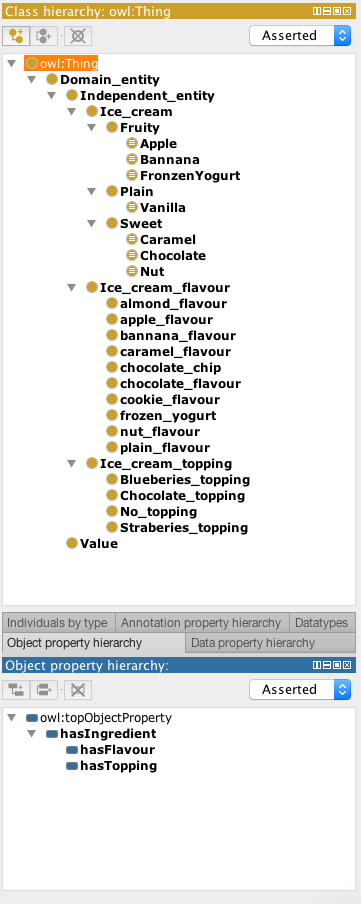
\includegraphics[width=260px]{img/class_and_properties.png}
      \caption{Sistemos objektai ir parametrai}
      \label{img:sistemos_objektai_ir_parametrai}
    \end{figure}

    \begin{figure}
      \centering
      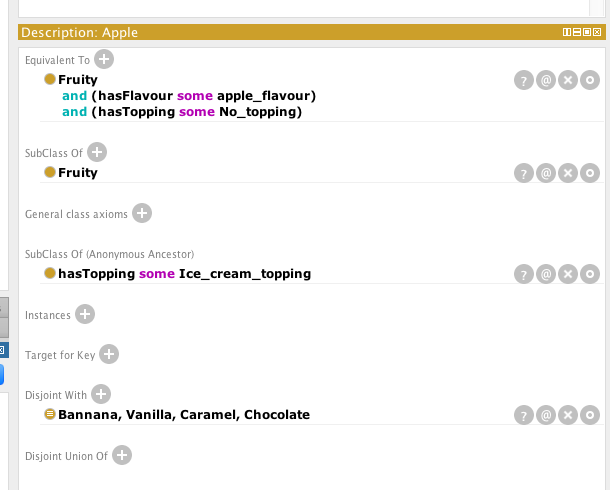
\includegraphics[width=360px]{img/apple.png}
      \caption{``Apple'' objektas}
      \label{img:appl_objektas}
    \end{figure}

    Tokiu būdu yra aprašoma ontologija Protege programoje.

    \section{Išvados}

    Darbo metu buvo išmoka dirbti su Protege programa, sudaryta ontologija. Iš viso sudarytas 31 objektas, kurie turi didžiausią 3 savybių skaičių.

\end{document}
